\documentclass{article}
\usepackage{graphicx} % Required for the inclusion of images
\usepackage{natbib} % Required to change bibliography style to APA
\usepackage{amsmath} % Required for some math elements 
\usepackage{wrapfig}
\usepackage{libertine} 
\usepackage{float}
\usepackage{listings}
\usepackage[skip=0pt]{caption}
\usepackage{float}
\usepackage[a4paper, margin=1in]{geometry}
\setlength\parindent{0pt} % Removes all indentation from paragraphs

\renewcommand{\today}{\ifcase \month \or January\or February\or March\or %
April\or May \or June\or July\or August\or September\or October\or November\or %
December\fi, \number \year} 
\renewcommand{\labelenumi}{\alph{enumi}.} % Make numbering in the enumerate environment by letter rather than number (e.g. section 6)

%\usepackage{times} % Uncomment to use the Times New Roman font

\title{Neural Networks and Deep Learning \\ Homework 1: Supervised Deep Learning}

\author{Giulio \textsc{Zani}} % Author name


\begin{document}

\maketitle % Insert the title, author and date


\tableofcontents


\section{Regression Task}
\subsection{Introduction}
For this task, we were given two files, one containin the train dataset and the other one the test datset. Both files containing a list of (x, y) couples. 
\begin{figure}[H]
  \begin{center}
    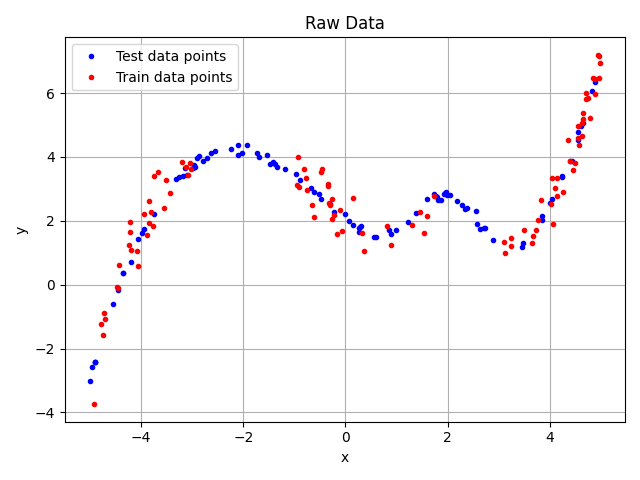
\includegraphics[width=\linewidth]{regression_task/imgs/raw_data.png}
    \caption{Raw data given for regression task}\label{raw_data}
  \end{center}
\end{figure}


As one may notice from the figure, the challenging part of task consists of ensuring that the model correctly guesses the function in those regions not represented by train data points 
(red in \figurename{\ref{raw_data}})

\subsection{Method}

For this task I have tried out a variety of settings by hand. This is the network structure:
\begin{lstlisting}
Net(
  (fc1): Linear(in_features=1, out_features=100, bias=True)
  (fc3): Linear(in_features=100, out_features=1, bias=True)
)
\end{lstlisting}

I have used a sigmoid activation function, without activation function in the output layer since this is a regression task.
As an optimizer I have used vanilla stochastic gradient descend algorithm (SGD). I have used a cross-validation training setup. Given that training for this task didn't take long, I decided to progressively keep track of the test loss as well (\figurename{\ref{test_loss}})

\begin{figure}[H]
    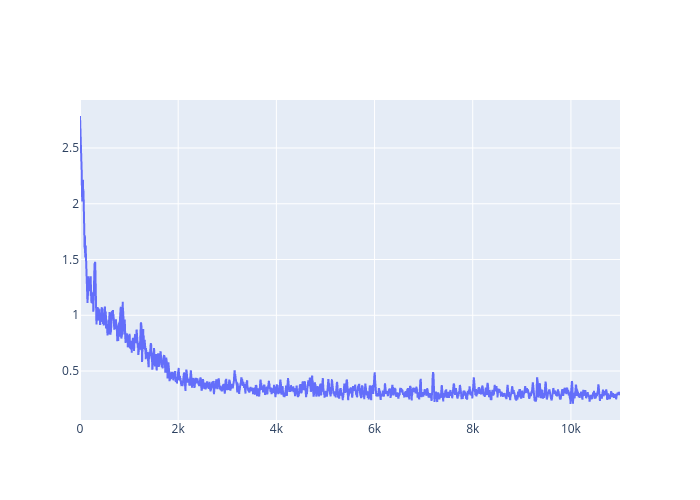
\includegraphics[width=\linewidth]{regression_task/imgs/val_loss.png}
    \caption{Validation loss as a function of the epoch (smoothed)}\label{val_loss}
\end{figure}
\begin{figure}[H]
    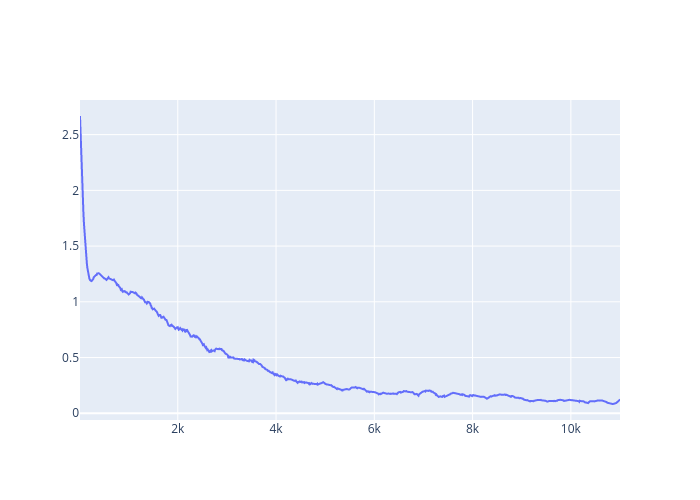
\includegraphics[width=\linewidth]{regression_task/imgs/test_loss.png}
    \caption{Test loss a function of the epoch (smoothed)}\label{test_loss}
\end{figure}

As one can see validation loss and test loss are both (roughly) monotonically decreasing, which is a good sign that the model is not overfitting. The model was trained for 1200 epochs, I have picked this number simply because I have observed that training for longer did not improve loss. The cross-validation is of 10 folds and a batch size of 9. As a loss funciton I have picked MSELoss, which implements mean square error (squared L2 norm) between each element in the input x and target y.
Code can be run with the following command:
\begin{lstlisting}
python -m deep_learning_hw1.regression_task
\end{lstlisting}

\subsection{Result}
\begin{figure}[H]
    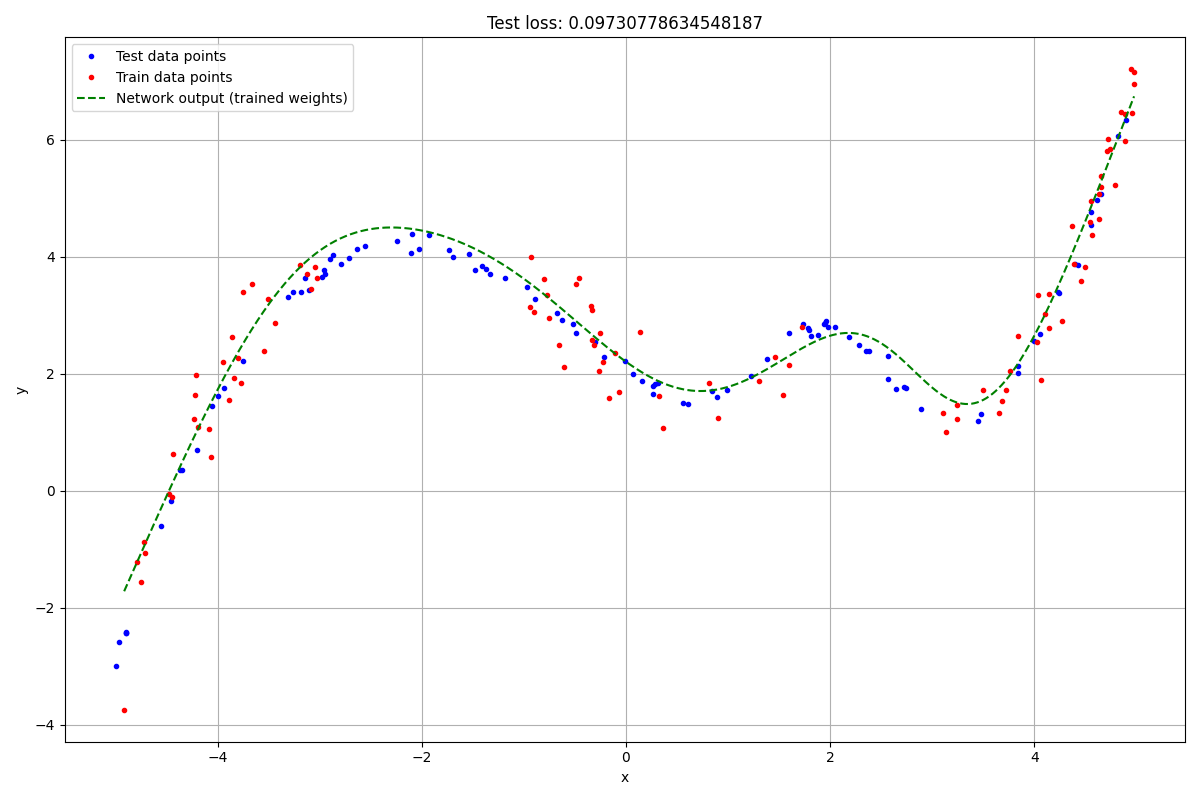
\includegraphics[width=\linewidth]{regression_task/imgs/model_and_data.png}
    \caption{Trained model plotted against raw data}\label{model_and_data}
\end{figure}
The mean final test loss was of 0.097. As one can see from \figurename{\ref{model_and_data}} the model has approximated pretty well the function even in those regions that were not included in the training set.

\section{Classification Task}
\subsection{Introduction}
In this taks we were given a dataset (MNIST) composed of images of handwritten digits. The deep model's objective is to learn to correctly classify the image to the corresponding image. Images are grayscale, 28x28 pixel.

\begin{figure}[H]
  \begin{center}
    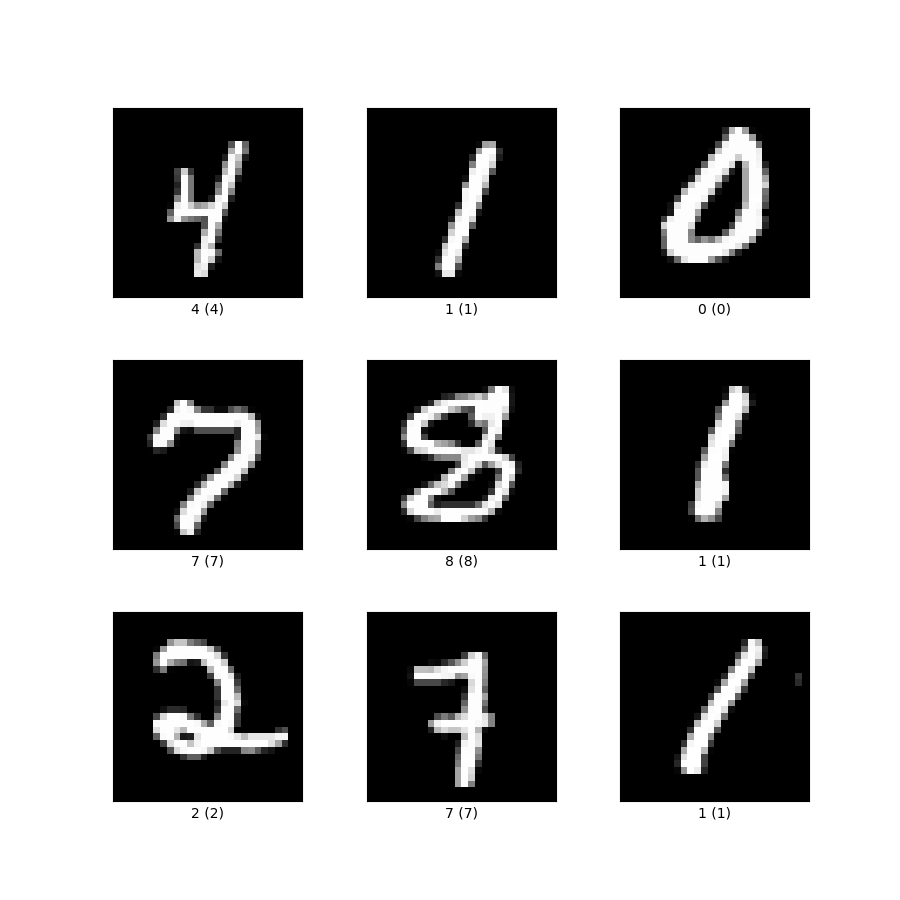
\includegraphics[width=10cm]{mnist_task/imgs/mnist_raw_data.png}
    \caption{Raw data given for regression task}\label{mnist_raw_data}
  \end{center}
\end{figure}

While the regression task can be better solved via methods that don't use deep learning, such as polynomial regression, this one canonically requires deep models. 

\subsection{Method}
Due to the relative small size of the input images, a simple, fully connected feed-farward ANN would suffice to solve the task pretty well. However I wanted to experiment with convolutional neural networks (CNNs). I have started out with a tutorial I have found on the internet.
\begin{lstlisting}
Net(
  (conv1): Conv2d(1, 32, kernel_size=(3, 3), stride=(1, 1))
  (conv2): Conv2d(32, 64, kernel_size=(3, 3), stride=(1, 1))
  (dropout1): Dropout(p=0.25, inplace=False)
  (dropout2): Dropout(p=0.5, inplace=False)
  (fc1): Linear(in_features=9216, out_features=128, bias=True)
  (fc2): Linear(in_features=128, out_features=10, bias=True)
)
\end{lstlisting}
I mainly fine-tuned this model by hand. I chose the dropout of 0.25 because it seems like this is a canonical value for CNNs. I have used ReLU activation function. I choose to use Adadelta optimizer because I have seen it in a tutorial, so I read about it and decided to used it. I have found it to be beneficial with respect to vanilla SGD.

\subsubsection{Optimizing Hyperparameters with Genetic Algorithm}
Genetic algorihms (GAs) are widely used to optimize hyperparameters, network structure and, more recently, deep learning algorihms. I have implemented a very simple tools to optimize hyperparameters using a GA. The algorithm performs both crossover and mutation. I meant to build this as a tool which I would use also in other exercises (such as homework 2), therefore, the tool doesn't assume anything about the nature of the problem, rather, it delegates the implementation of a few functions, namely: "mutate", "get random genome" and "get fitness". In this particular problem to compute an organism's fitness, I have run a training for one epoch with the given genome/parameters and returned the test loss (which actually would be the fitness' inverse). I am a little concerned about whether computing the fitness based only of a one-epoch training could introduce a bias in hyperparameters search, however I had no choice due to limited hardware availability.
The initial population size is of 30, and I have run this for 28 generations. The hyperparameters over wich I run it were the following:

$$
\textrm{batch size} \in \{10,...,128\}
$$
$$
\textrm{lr} \in [1e-8, 1.0]
$$
$$
\textrm{gamma} \in [0, 1.0]
$$
$$
\textrm{weight decay} \in [1e-7, 1e-4]
$$

The evolved hyperparameters are:
$$
\textrm{batch size} = 10
$$
$$
\textrm{lr} = 0.419
$$
$$
\textrm{gamma} =  0.8366
$$
$$
\textrm{weight decay} = 7.511239e-05
$$

\begin{figure}[H]
    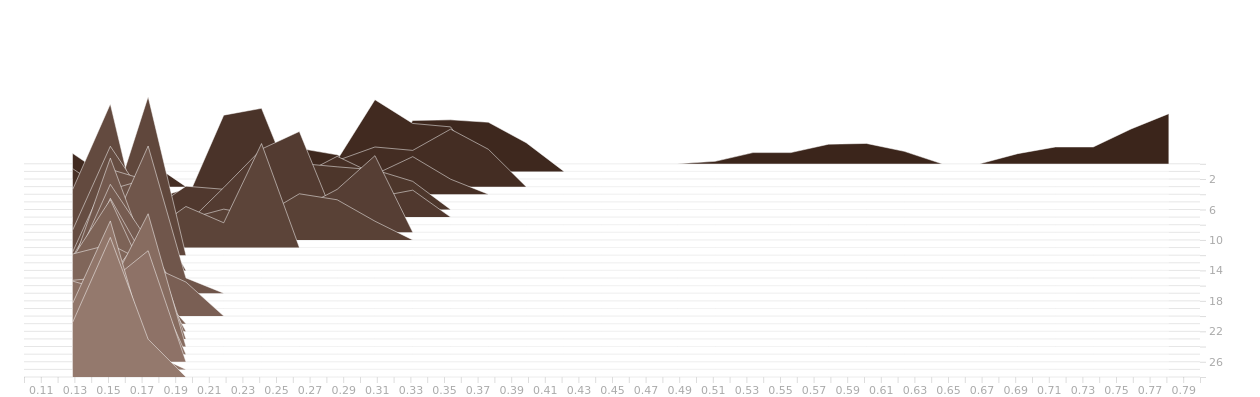
\includegraphics[width=\linewidth]{mnist_task/imgs/genetic_population_2.png}
    \caption{Distribution of 30\% best individuals after each generation. One-epoch loss on y axis.}\label{best_fitness}
\end{figure}
With more time and computational resources it would have been interesting to explore network structure optimization.

\subsubsection{Training and network analysis}
Here I have traced the loss during training. In the second plot I have taken the test set because my first version was not using a (cross)validation set.
\begin{figure}[H]
    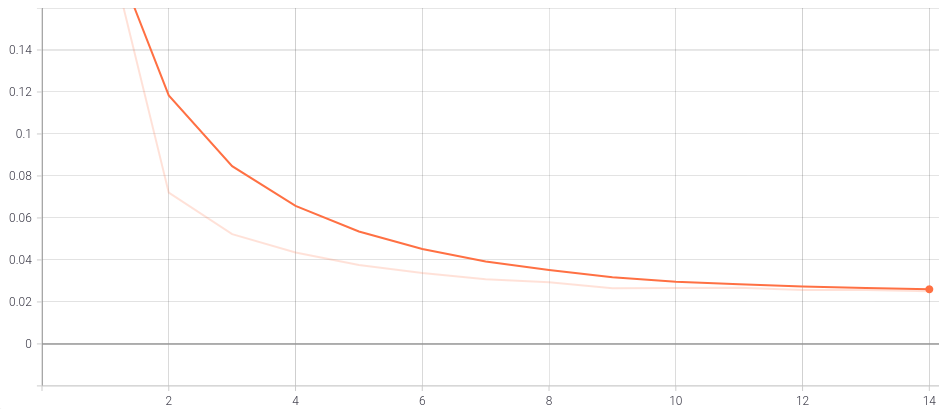
\includegraphics[width=\linewidth]{mnist_task/imgs/train_loss.png}
    \caption{Training loss as a function of the epoch}\label{conv1}
\end{figure}
\begin{figure}[H]
    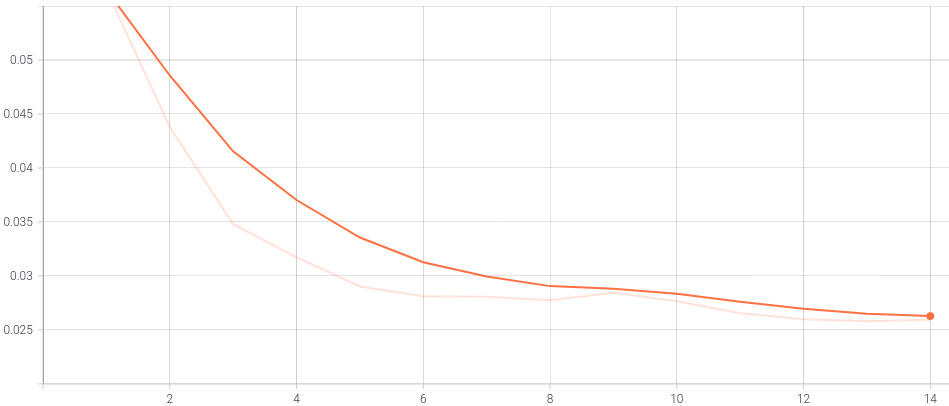
\includegraphics[width=\linewidth]{mnist_task/imgs/test_loss.png}
    \caption{Test loss as a function of the epoch}\label{conv1}
\end{figure}

I have used a pytorch hook to plot the activation of the firs conolutional layer. And with tensorboard I have plotted its weights distribution over the epoch.
\begin{figure}[H]
    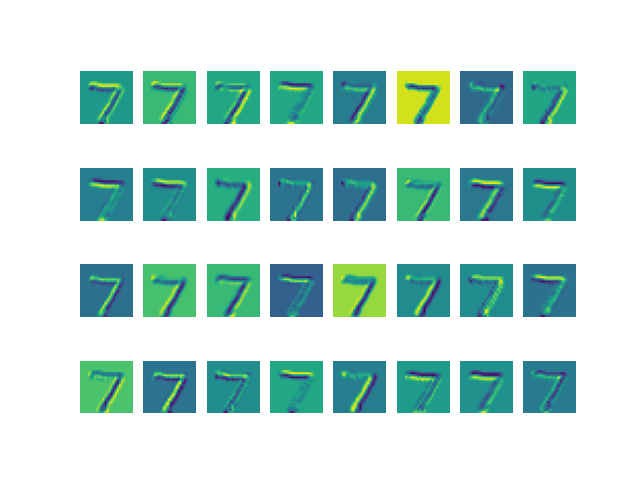
\includegraphics[width=\linewidth]{mnist_task/imgs/conv1.png}
    \caption{Activation of network's first convolutional layer (one image per channel)}\label{conv1}
\end{figure}
\begin{figure}[H]
    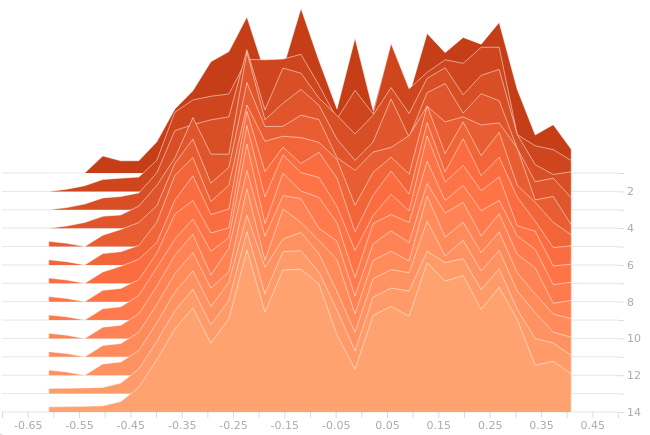
\includegraphics[width=\linewidth]{mnist_task/imgs/conv1_weight_dist.png}
    \caption{First convolutional layer weights distribution at every epoch}\label{conv1}
\end{figure}


\subsection{Result}
In the final test set the average loss was of 0.0268 and the accuracy of 9917/10000=99.17\%
\end{document}
